\documentclass[1p]{elsarticle_modified}
%\bibliographystyle{elsarticle-num}

%\usepackage[colorlinks]{hyperref}
%\usepackage{abbrmath_seonhwa} %\Abb, \Ascr, \Acal ,\Abf, \Afrak
\usepackage{amsfonts}
\usepackage{amssymb}
\usepackage{amsmath}
\usepackage{amsthm}
\usepackage{scalefnt}
\usepackage{amsbsy}
\usepackage{kotex}
\usepackage{caption}
\usepackage{subfig}
\usepackage{color}
\usepackage{graphicx}
\usepackage{xcolor} %% white, black, red, green, blue, cyan, magenta, yellow
\usepackage{float}
\usepackage{setspace}
\usepackage{hyperref}

\usepackage{tikz}
\usetikzlibrary{arrows}

\usepackage{multirow}
\usepackage{array} % fixed length table
\usepackage{hhline}

%%%%%%%%%%%%%%%%%%%%%
\makeatletter
\renewcommand*\env@matrix[1][\arraystretch]{%
	\edef\arraystretch{#1}%
	\hskip -\arraycolsep
	\let\@ifnextchar\new@ifnextchar
	\array{*\c@MaxMatrixCols c}}
\makeatother %https://tex.stackexchange.com/questions/14071/how-can-i-increase-the-line-spacing-in-a-matrix
%%%%%%%%%%%%%%%

\usepackage[normalem]{ulem}

\newcommand{\msout}[1]{\ifmmode\text{\sout{\ensuremath{#1}}}\else\sout{#1}\fi}
%SOURCE: \msout is \stkout macro in https://tex.stackexchange.com/questions/20609/strikeout-in-math-mode

\newcommand{\cancel}[1]{
	\ifmmode
	{\color{red}\msout{#1}}
	\else
	{\color{red}\sout{#1}}
	\fi
}

\newcommand{\add}[1]{
	{\color{blue}\uwave{#1}}
}

\newcommand{\replace}[2]{
	\ifmmode
	{\color{red}\msout{#1}}{\color{blue}\uwave{#2}}
	\else
	{\color{red}\sout{#1}}{\color{blue}\uwave{#2}}
	\fi
}

\newcommand{\Sol}{\mathcal{S}} %segment
\newcommand{\D}{D} %diagram
\newcommand{\A}{\mathcal{A}} %arc


%%%%%%%%%%%%%%%%%%%%%%%%%%%%%5 test

\def\sl{\operatorname{\textup{SL}}(2,\Cbb)}
\def\psl{\operatorname{\textup{PSL}}(2,\Cbb)}
\def\quan{\mkern 1mu \triangleright \mkern 1mu}

\theoremstyle{definition}
\newtheorem{thm}{Theorem}[section]
\newtheorem{prop}[thm]{Proposition}
\newtheorem{lem}[thm]{Lemma}
\newtheorem{ques}[thm]{Question}
\newtheorem{cor}[thm]{Corollary}
\newtheorem{defn}[thm]{Definition}
\newtheorem{exam}[thm]{Example}
\newtheorem{rmk}[thm]{Remark}
\newtheorem{alg}[thm]{Algorithm}

\newcommand{\I}{\sqrt{-1}}
\begin{document}

%\begin{frontmatter}
%
%\title{Boundary parabolic representations of knots up to 8 crossings}
%
%%% Group authors per affiliation:
%\author{Yunhi Cho} 
%\address{Department of Mathematics, University of Seoul, Seoul, Korea}
%\ead{yhcho@uos.ac.kr}
%
%
%\author{Seonhwa Kim} %\fnref{s_kim}}
%\address{Center for Geometry and Physics, Institute for Basic Science, Pohang, 37673, Korea}
%\ead{ryeona17@ibs.re.kr}
%
%\author{Hyuk Kim}
%\address{Department of Mathematical Sciences, Seoul National University, Seoul 08826, Korea}
%\ead{hyukkim@snu.ac.kr}
%
%\author{Seokbeom Yoon}
%\address{Department of Mathematical Sciences, Seoul National University, Seoul, 08826,  Korea}
%\ead{sbyoon15@snu.ac.kr}
%
%\begin{abstract}
%We find all boundary parabolic representation of knots up to 8 crossings.
%
%\end{abstract}
%\begin{keyword}
%    \MSC[2010] 57M25 
%\end{keyword}
%
%\end{frontmatter}

%\linenumbers
%\tableofcontents
%
\newcommand\colored[1]{\textcolor{white}{\rule[-0.35ex]{0.8em}{1.4ex}}\kern-0.8em\color{red} #1}%
%\newcommand\colored[1]{\textcolor{white}{ #1}\kern-2.17ex	\textcolor{white}{ #1}\kern-1.81ex	\textcolor{white}{ #1}\kern-2.15ex\color{red}#1	}

{\Large $\underline{11a_{268}~(K11a_{268})}$}

\setlength{\tabcolsep}{10pt}
\renewcommand{\arraystretch}{1.6}
\vspace{1cm}\begin{tabular}{m{100pt}>{\centering\arraybackslash}m{274pt}}
\multirow{5}{120pt}{
	\centering
	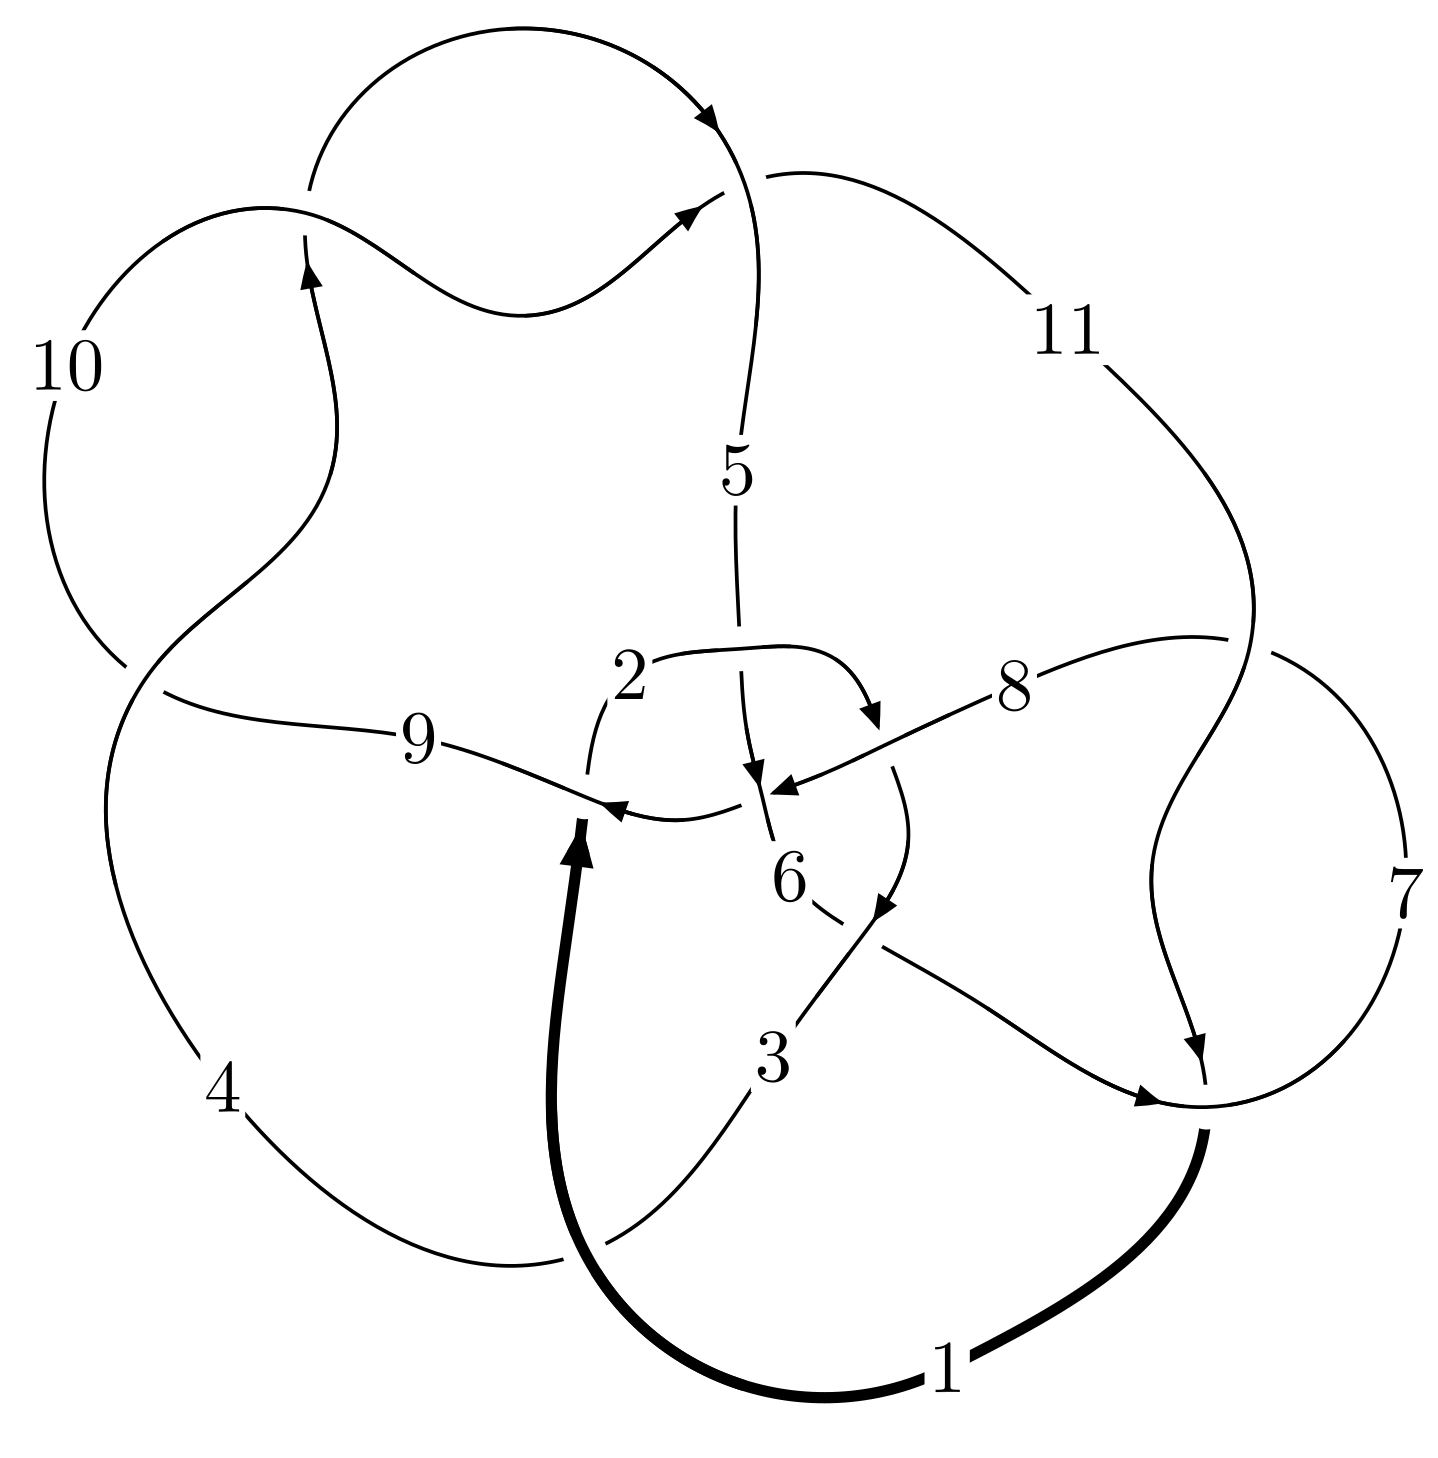
\includegraphics[width=112pt]{../../../GIT/diagram.site/Diagrams/png/517_11a_268.png}\\
\ \ \ A knot diagram\footnotemark}&
\allowdisplaybreaks
\textbf{Linearized knot diagam} \\
\cline{2-2}
 &
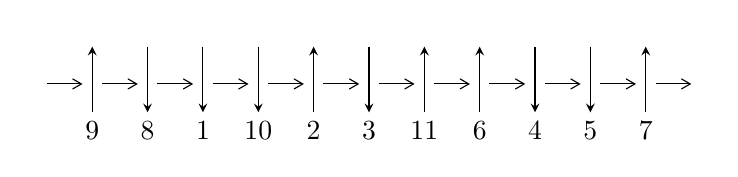
\begin{tikzpicture}[x=20pt, y=17pt]
	% nodes
	\node (C0) at (0, 0) {};
	\node (C1) at (1, 0) {};
	\node (C1U) at (1, +1) {};
	\node (C1D) at (1, -1) {9};

	\node (C2) at (2, 0) {};
	\node (C2U) at (2, +1) {};
	\node (C2D) at (2, -1) {8};

	\node (C3) at (3, 0) {};
	\node (C3U) at (3, +1) {};
	\node (C3D) at (3, -1) {1};

	\node (C4) at (4, 0) {};
	\node (C4U) at (4, +1) {};
	\node (C4D) at (4, -1) {10};

	\node (C5) at (5, 0) {};
	\node (C5U) at (5, +1) {};
	\node (C5D) at (5, -1) {2};

	\node (C6) at (6, 0) {};
	\node (C6U) at (6, +1) {};
	\node (C6D) at (6, -1) {3};

	\node (C7) at (7, 0) {};
	\node (C7U) at (7, +1) {};
	\node (C7D) at (7, -1) {11};

	\node (C8) at (8, 0) {};
	\node (C8U) at (8, +1) {};
	\node (C8D) at (8, -1) {6};

	\node (C9) at (9, 0) {};
	\node (C9U) at (9, +1) {};
	\node (C9D) at (9, -1) {4};

	\node (C10) at (10, 0) {};
	\node (C10U) at (10, +1) {};
	\node (C10D) at (10, -1) {5};

	\node (C11) at (11, 0) {};
	\node (C11U) at (11, +1) {};
	\node (C11D) at (11, -1) {7};
	\node (C12) at (12, 0) {};

	% arrows
	\draw[->,>={angle 60}]
	(C0) edge (C1) (C1) edge (C2) (C2) edge (C3) (C3) edge (C4) (C4) edge (C5) (C5) edge (C6) (C6) edge (C7) (C7) edge (C8) (C8) edge (C9) (C9) edge (C10) (C10) edge (C11) (C11) edge (C12) ;	\draw[->,>=stealth]
	(C1D) edge (C1U) (C2U) edge (C2D) (C3U) edge (C3D) (C4U) edge (C4D) (C5D) edge (C5U) (C6U) edge (C6D) (C7D) edge (C7U) (C8D) edge (C8U) (C9U) edge (C9D) (C10U) edge (C10D) (C11D) edge (C11U) ;
	\end{tikzpicture} \\
\hhline{~~} \\& 
\textbf{Solving Sequence} \\ \cline{2-2} 
 &
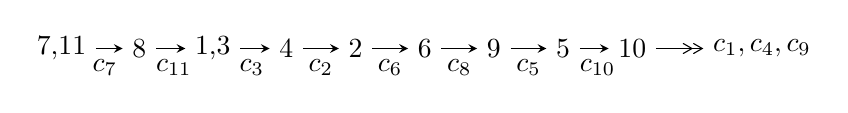
\begin{tikzpicture}[x=25pt, y=7pt]
	% node
	\node (A0) at (-1/8, 0) {7,11};
	\node (A1) at (1, 0) {8};
	\node (A2) at (33/16, 0) {1,3};
	\node (A3) at (25/8, 0) {4};
	\node (A4) at (33/8, 0) {2};
	\node (A5) at (41/8, 0) {6};
	\node (A6) at (49/8, 0) {9};
	\node (A7) at (57/8, 0) {5};
	\node (A8) at (65/8, 0) {10};
	\node (C1) at (1/2, -1) {$c_{7}$};
	\node (C2) at (3/2, -1) {$c_{11}$};
	\node (C3) at (21/8, -1) {$c_{3}$};
	\node (C4) at (29/8, -1) {$c_{2}$};
	\node (C5) at (37/8, -1) {$c_{6}$};
	\node (C6) at (45/8, -1) {$c_{8}$};
	\node (C7) at (53/8, -1) {$c_{5}$};
	\node (C8) at (61/8, -1) {$c_{10}$};
	\node (A9) at (10, 0) {$c_{1},c_{4},c_{9}$};

	% edge
	\draw[->,>=stealth]	
	(A0) edge (A1) (A1) edge (A2) (A2) edge (A3) (A3) edge (A4) (A4) edge (A5) (A5) edge (A6) (A6) edge (A7) (A7) edge (A8) ;
	\draw[->>,>={angle 60}]	
	(A8) edge (A9);
\end{tikzpicture} \\ 

\end{tabular} \\

\footnotetext{
The image of knot diagram is generated by the software ``\textbf{Draw programme}" developed by Andrew Bartholomew(\url{http://www.layer8.co.uk/maths/draw/index.htm\#Running-draw}), where we modified some parts for our purpose(\url{https://github.com/CATsTAILs/LinksPainter}).
}\phantom \\ \newline 
\centering \textbf{Ideals for irreducible components\footnotemark of $X_{\text{par}}$} 
 
\begin{align*}
I^u_{1}&=\langle 
-2.49863\times10^{257} u^{88}+5.28339\times10^{257} u^{87}+\cdots+2.06470\times10^{257} b+1.62471\times10^{259},\\
\phantom{I^u_{1}}&\phantom{= \langle  }-1.46587\times10^{259} u^{88}+5.63526\times10^{259} u^{87}+\cdots+1.21817\times10^{259} a+2.14864\times10^{261},\\
\phantom{I^u_{1}}&\phantom{= \langle  }u^{89}- u^{88}+\cdots+48 u+59\rangle \\
I^u_{2}&=\langle 
u^{18}-2 u^{17}+\cdots+b-1,\;2810 u^{19}-4920 u^{18}+\cdots+107 a-1193,\;u^{20}-2 u^{19}+\cdots+u-1\rangle \\
\\
\end{align*}
\raggedright * 2 irreducible components of $\dim_{\mathbb{C}}=0$, with total 109 representations.\\
\footnotetext{All coefficients of polynomials are rational numbers. But the coefficients are sometimes approximated in decimal forms when there is not enough margin.}
\newpage
\renewcommand{\arraystretch}{1}
\centering \section*{I. $I^u_{1}= \langle -2.50\times10^{257} u^{88}+5.28\times10^{257} u^{87}+\cdots+2.06\times10^{257} b+1.62\times10^{259},\;-1.47\times10^{259} u^{88}+5.64\times10^{259} u^{87}+\cdots+1.22\times10^{259} a+2.15\times10^{261},\;u^{89}- u^{88}+\cdots+48 u+59 \rangle$}
\flushleft \textbf{(i) Arc colorings}\\
\begin{tabular}{m{7pt} m{180pt} m{7pt} m{180pt} }
\flushright $a_{7}=$&$\begin{pmatrix}1\\0\end{pmatrix}$ \\
\flushright $a_{11}=$&$\begin{pmatrix}0\\u\end{pmatrix}$ \\
\flushright $a_{8}=$&$\begin{pmatrix}1\\- u^2\end{pmatrix}$ \\
\flushright $a_{1}=$&$\begin{pmatrix}u\\u\end{pmatrix}$ \\
\flushright $a_{3}=$&$\begin{pmatrix}1.20333 u^{88}-4.62599 u^{87}+\cdots-65.4798 u-176.382\\1.21016 u^{88}-2.55892 u^{87}+\cdots-4.73499 u-78.6901\end{pmatrix}$ \\
\flushright $a_{4}=$&$\begin{pmatrix}1.19352 u^{88}-2.15965 u^{87}+\cdots+34.4706 u-54.0216\\1.20035 u^{88}-0.0925750 u^{87}+\cdots+95.2154 u+43.6703\end{pmatrix}$ \\
\flushright $a_{2}=$&$\begin{pmatrix}0.866135 u^{88}-1.82355 u^{87}+\cdots+23.0760 u-53.1353\\0.669502 u^{88}+0.854257 u^{87}+\cdots+93.7021 u+66.7594\end{pmatrix}$ \\
\flushright $a_{6}=$&$\begin{pmatrix}-1.85198 u^{88}+1.84275 u^{87}+\cdots-99.2054 u+21.2049\\-1.38144 u^{88}+0.574780 u^{87}+\cdots-104.158 u-29.9703\end{pmatrix}$ \\
\flushright $a_{9}=$&$\begin{pmatrix}-0.161350 u^{88}-1.91766 u^{87}+\cdots-107.928 u-102.769\\1.27346 u^{88}-2.34459 u^{87}+\cdots+9.19607 u-60.8438\end{pmatrix}$ \\
\flushright $a_{5}=$&$\begin{pmatrix}-1.27022 u^{88}+0.255281 u^{87}+\cdots-89.4254 u-49.1154\\-1.92719 u^{88}+0.959452 u^{87}+\cdots-136.691 u-46.0116\end{pmatrix}$ \\
\flushright $a_{10}=$&$\begin{pmatrix}-0.293092 u^{88}-0.892600 u^{87}+\cdots-95.2003 u-56.2570\\0.191137 u^{88}+1.45973 u^{87}+\cdots+91.9737 u+92.2085\end{pmatrix}$\\ \flushright $a_{10}=$&$\begin{pmatrix}-0.293092 u^{88}-0.892600 u^{87}+\cdots-95.2003 u-56.2570\\0.191137 u^{88}+1.45973 u^{87}+\cdots+91.9737 u+92.2085\end{pmatrix}$\\&\end{tabular}
\flushleft \textbf{(ii) Obstruction class $= -1$}\\~\\
\flushleft \textbf{(iii) Cusp Shapes $= 0.667960 u^{88}+1.19445 u^{87}+\cdots+98.6923 u+70.3629$}\\~\\
\newpage\renewcommand{\arraystretch}{1}
\flushleft \textbf{(iv) u-Polynomials at the component}\newline \\
\begin{tabular}{m{50pt}|m{274pt}}
Crossings & \hspace{64pt}u-Polynomials at each crossing \\
\hline $$\begin{aligned}c_{1}\end{aligned}$$&$\begin{aligned}
&u^{89}-4 u^{88}+\cdots-121118 u-30299
\end{aligned}$\\
\hline $$\begin{aligned}c_{2}\end{aligned}$$&$\begin{aligned}
&u^{89}- u^{88}+\cdots+74 u-3
\end{aligned}$\\
\hline $$\begin{aligned}c_{3}\end{aligned}$$&$\begin{aligned}
&u^{89}+6 u^{88}+\cdots+9173 u-3187
\end{aligned}$\\
\hline $$\begin{aligned}c_{4},c_{9},c_{10}\end{aligned}$$&$\begin{aligned}
&u^{89}-45 u^{87}+\cdots-29 u+1
\end{aligned}$\\
\hline $$\begin{aligned}c_{5}\end{aligned}$$&$\begin{aligned}
&u^{89}+5 u^{87}+\cdots-1510 u-191
\end{aligned}$\\
\hline $$\begin{aligned}c_{6}\end{aligned}$$&$\begin{aligned}
&u^{89}+u^{88}+\cdots+84 u-2543
\end{aligned}$\\
\hline $$\begin{aligned}c_{7},c_{11}\end{aligned}$$&$\begin{aligned}
&u^{89}+u^{88}+\cdots+48 u-59
\end{aligned}$\\
\hline $$\begin{aligned}c_{8}\end{aligned}$$&$\begin{aligned}
&u^{89}+8 u^{88}+\cdots+21 u+1
\end{aligned}$\\
\hline
\end{tabular}\\~\\
\newpage\renewcommand{\arraystretch}{1}
\flushleft \textbf{(v) Riley Polynomials at the component}\newline \\
\begin{tabular}{m{50pt}|m{274pt}}
Crossings & \hspace{64pt}Riley Polynomials at each crossing \\
\hline $$\begin{aligned}c_{1}\end{aligned}$$&$\begin{aligned}
&y^{89}+22 y^{88}+\cdots-31326433006 y-918029401
\end{aligned}$\\
\hline $$\begin{aligned}c_{2}\end{aligned}$$&$\begin{aligned}
&y^{89}-7 y^{88}+\cdots+1222 y-9
\end{aligned}$\\
\hline $$\begin{aligned}c_{3}\end{aligned}$$&$\begin{aligned}
&y^{89}-40 y^{88}+\cdots+740124139 y-10156969
\end{aligned}$\\
\hline $$\begin{aligned}c_{4},c_{9},c_{10}\end{aligned}$$&$\begin{aligned}
&y^{89}-90 y^{88}+\cdots+123 y-1
\end{aligned}$\\
\hline $$\begin{aligned}c_{5}\end{aligned}$$&$\begin{aligned}
&y^{89}+10 y^{88}+\cdots-1020380 y-36481
\end{aligned}$\\
\hline $$\begin{aligned}c_{6}\end{aligned}$$&$\begin{aligned}
&y^{89}-17 y^{88}+\cdots+242227806 y-6466849
\end{aligned}$\\
\hline $$\begin{aligned}c_{7},c_{11}\end{aligned}$$&$\begin{aligned}
&y^{89}+57 y^{88}+\cdots-106492 y-3481
\end{aligned}$\\
\hline $$\begin{aligned}c_{8}\end{aligned}$$&$\begin{aligned}
&y^{89}+12 y^{88}+\cdots+29 y-1
\end{aligned}$\\
\hline
\end{tabular}\\~\\
\newpage\flushleft \textbf{(vi) Complex Volumes and Cusp Shapes}
$$\begin{array}{c|c|c}  
\text{Solutions to }I^u_{1}& \I (\text{vol} + \sqrt{-1}CS) & \text{Cusp shape}\\
 \hline 
\begin{aligned}
u &= \phantom{-}0.087265 + 0.982767 I \\
a &= -0.04086 - 1.58758 I \\
b &= -0.19737 - 2.33544 I\end{aligned}
 & -0.50502 + 3.23925 I & \phantom{-0.000000 } 0 \\ \hline\begin{aligned}
u &= \phantom{-}0.087265 - 0.982767 I \\
a &= -0.04086 + 1.58758 I \\
b &= -0.19737 + 2.33544 I\end{aligned}
 & -0.50502 - 3.23925 I & \phantom{-0.000000 } 0 \\ \hline\begin{aligned}
u &= \phantom{-}0.046780 + 1.013680 I \\
a &= \phantom{-}0.416851 - 0.354974 I \\
b &= -0.111187 + 1.159690 I\end{aligned}
 & -3.50317 + 2.78548 I & \phantom{-0.000000 } 0 \\ \hline\begin{aligned}
u &= \phantom{-}0.046780 - 1.013680 I \\
a &= \phantom{-}0.416851 + 0.354974 I \\
b &= -0.111187 - 1.159690 I\end{aligned}
 & -3.50317 - 2.78548 I & \phantom{-0.000000 } 0 \\ \hline\begin{aligned}
u &= -0.446021 + 0.914047 I \\
a &= -2.48559 + 0.54321 I \\
b &= -0.571797 - 0.795448 I\end{aligned}
 & -5.19564 - 7.48572 I & \phantom{-0.000000 } 0 \\ \hline\begin{aligned}
u &= -0.446021 - 0.914047 I \\
a &= -2.48559 - 0.54321 I \\
b &= -0.571797 + 0.795448 I\end{aligned}
 & -5.19564 + 7.48572 I & \phantom{-0.000000 } 0 \\ \hline\begin{aligned}
u &= \phantom{-}0.260416 + 1.013500 I \\
a &= \phantom{-}2.27900 - 0.32057 I \\
b &= \phantom{-}0.659896 - 0.535201 I\end{aligned}
 & -0.59074 + 5.03975 I & \phantom{-0.000000 } 0 \\ \hline\begin{aligned}
u &= \phantom{-}0.260416 - 1.013500 I \\
a &= \phantom{-}2.27900 + 0.32057 I \\
b &= \phantom{-}0.659896 + 0.535201 I\end{aligned}
 & -0.59074 - 5.03975 I & \phantom{-0.000000 } 0 \\ \hline\begin{aligned}
u &= \phantom{-}1.064020 + 0.063310 I \\
a &= \phantom{-}0.045029 - 0.215883 I \\
b &= -0.911465 - 0.659115 I\end{aligned}
 & -0.03232 - 7.23979 I & \phantom{-0.000000 } 0 \\ \hline\begin{aligned}
u &= \phantom{-}1.064020 - 0.063310 I \\
a &= \phantom{-}0.045029 + 0.215883 I \\
b &= -0.911465 + 0.659115 I\end{aligned}
 & -0.03232 + 7.23979 I & \phantom{-0.000000 } 0\\
 \hline 
 \end{array}$$\newpage$$\begin{array}{c|c|c}  
\text{Solutions to }I^u_{1}& \I (\text{vol} + \sqrt{-1}CS) & \text{Cusp shape}\\
 \hline 
\begin{aligned}
u &= \phantom{-}0.039185 + 1.073690 I \\
a &= -1.47979 - 1.15466 I \\
b &= -0.627270 - 0.234640 I\end{aligned}
 & -3.66917 - 2.24819 I & \phantom{-0.000000 } 0 \\ \hline\begin{aligned}
u &= \phantom{-}0.039185 - 1.073690 I \\
a &= -1.47979 + 1.15466 I \\
b &= -0.627270 + 0.234640 I\end{aligned}
 & -3.66917 + 2.24819 I & \phantom{-0.000000 } 0 \\ \hline\begin{aligned}
u &= \phantom{-}0.497647 + 0.954960 I \\
a &= \phantom{-}1.28701 + 0.60287 I \\
b &= \phantom{-}0.477386 + 0.066075 I\end{aligned}
 & -4.69329 + 4.27856 I & \phantom{-0.000000 } 0 \\ \hline\begin{aligned}
u &= \phantom{-}0.497647 - 0.954960 I \\
a &= \phantom{-}1.28701 - 0.60287 I \\
b &= \phantom{-}0.477386 - 0.066075 I\end{aligned}
 & -4.69329 - 4.27856 I & \phantom{-0.000000 } 0 \\ \hline\begin{aligned}
u &= \phantom{-}0.039765 + 1.076270 I \\
a &= \phantom{-}1.46166 + 0.75014 I \\
b &= \phantom{-}1.017060 - 0.460738 I\end{aligned}
 & -4.07004 + 0.47327 I & \phantom{-0.000000 } 0 \\ \hline\begin{aligned}
u &= \phantom{-}0.039765 - 1.076270 I \\
a &= \phantom{-}1.46166 - 0.75014 I \\
b &= \phantom{-}1.017060 + 0.460738 I\end{aligned}
 & -4.07004 - 0.47327 I & \phantom{-0.000000 } 0 \\ \hline\begin{aligned}
u &= -0.615419 + 0.671458 I \\
a &= \phantom{-}0.189017 - 0.505603 I \\
b &= -0.560076 + 1.171310 I\end{aligned}
 & -4.51518 + 3.24714 I & \phantom{-0.000000 } 0 \\ \hline\begin{aligned}
u &= -0.615419 - 0.671458 I \\
a &= \phantom{-}0.189017 + 0.505603 I \\
b &= -0.560076 - 1.171310 I\end{aligned}
 & -4.51518 - 3.24714 I & \phantom{-0.000000 } 0 \\ \hline\begin{aligned}
u &= -0.121420 + 1.106610 I \\
a &= \phantom{-}1.31626 + 0.66629 I \\
b &= \phantom{-}1.031160 + 0.909995 I\end{aligned}
 & -1.75568 - 2.78654 I & \phantom{-0.000000 } 0 \\ \hline\begin{aligned}
u &= -0.121420 - 1.106610 I \\
a &= \phantom{-}1.31626 - 0.66629 I \\
b &= \phantom{-}1.031160 - 0.909995 I\end{aligned}
 & -1.75568 + 2.78654 I & \phantom{-0.000000 } 0\\
 \hline 
 \end{array}$$\newpage$$\begin{array}{c|c|c}  
\text{Solutions to }I^u_{1}& \I (\text{vol} + \sqrt{-1}CS) & \text{Cusp shape}\\
 \hline 
\begin{aligned}
u &= -0.875117 + 0.034580 I \\
a &= -0.386985 - 0.034842 I \\
b &= -0.155945 - 0.596885 I\end{aligned}
 & \phantom{-}2.36715 - 0.35769 I & \phantom{-0.000000 } 0 \\ \hline\begin{aligned}
u &= -0.875117 - 0.034580 I \\
a &= -0.386985 + 0.034842 I \\
b &= -0.155945 + 0.596885 I\end{aligned}
 & \phantom{-}2.36715 + 0.35769 I & \phantom{-0.000000 } 0 \\ \hline\begin{aligned}
u &= \phantom{-}1.007920 + 0.535449 I \\
a &= \phantom{-}0.336385 - 0.013362 I \\
b &= \phantom{-}0.531325 + 0.593484 I\end{aligned}
 & -2.70373 + 0.98079 I & \phantom{-0.000000 } 0 \\ \hline\begin{aligned}
u &= \phantom{-}1.007920 - 0.535449 I \\
a &= \phantom{-}0.336385 + 0.013362 I \\
b &= \phantom{-}0.531325 - 0.593484 I\end{aligned}
 & -2.70373 - 0.98079 I & \phantom{-0.000000 } 0 \\ \hline\begin{aligned}
u &= \phantom{-}0.506291 + 1.032270 I \\
a &= \phantom{-}0.866930 + 0.935334 I \\
b &= \phantom{-}1.191080 - 0.080568 I\end{aligned}
 & -3.66544 + 1.93275 I & \phantom{-0.000000 } 0 \\ \hline\begin{aligned}
u &= \phantom{-}0.506291 - 1.032270 I \\
a &= \phantom{-}0.866930 - 0.935334 I \\
b &= \phantom{-}1.191080 + 0.080568 I\end{aligned}
 & -3.66544 - 1.93275 I & \phantom{-0.000000 } 0 \\ \hline\begin{aligned}
u &= -0.236142 + 1.129110 I \\
a &= \phantom{-}0.330233 - 1.155500 I \\
b &= \phantom{-}0.70775 - 2.08057 I\end{aligned}
 & -7.96934 - 7.75557 I & \phantom{-0.000000 } 0 \\ \hline\begin{aligned}
u &= -0.236142 - 1.129110 I \\
a &= \phantom{-}0.330233 + 1.155500 I \\
b &= \phantom{-}0.70775 + 2.08057 I\end{aligned}
 & -7.96934 + 7.75557 I & \phantom{-0.000000 } 0 \\ \hline\begin{aligned}
u &= -0.328525 + 0.779440 I \\
a &= -0.807758 + 0.527555 I \\
b &= -0.410749 + 0.471628 I\end{aligned}
 & -0.12055 - 1.56154 I & \phantom{-0.000000 } 0 \\ \hline\begin{aligned}
u &= -0.328525 - 0.779440 I \\
a &= -0.807758 - 0.527555 I \\
b &= -0.410749 - 0.471628 I\end{aligned}
 & -0.12055 + 1.56154 I & \phantom{-0.000000 } 0\\
 \hline 
 \end{array}$$\newpage$$\begin{array}{c|c|c}  
\text{Solutions to }I^u_{1}& \I (\text{vol} + \sqrt{-1}CS) & \text{Cusp shape}\\
 \hline 
\begin{aligned}
u &= -0.788124 + 0.303926 I \\
a &= -0.387345 + 0.099692 I \\
b &= \phantom{-}0.619681 + 0.601987 I\end{aligned}
 & \phantom{-}0.06582 - 2.81820 I & \phantom{-0.000000 } 0 \\ \hline\begin{aligned}
u &= -0.788124 - 0.303926 I \\
a &= -0.387345 - 0.099692 I \\
b &= \phantom{-}0.619681 - 0.601987 I\end{aligned}
 & \phantom{-}0.06582 + 2.81820 I & \phantom{-0.000000 } 0 \\ \hline\begin{aligned}
u &= \phantom{-}0.445920 + 1.083550 I \\
a &= \phantom{-}1.87113 + 0.43186 I \\
b &= \phantom{-}1.44730 - 0.78897 I\end{aligned}
 & -3.75095 + 4.98969 I & \phantom{-0.000000 } 0 \\ \hline\begin{aligned}
u &= \phantom{-}0.445920 - 1.083550 I \\
a &= \phantom{-}1.87113 - 0.43186 I \\
b &= \phantom{-}1.44730 + 0.78897 I\end{aligned}
 & -3.75095 - 4.98969 I & \phantom{-0.000000 } 0 \\ \hline\begin{aligned}
u &= \phantom{-}0.678170 + 0.961510 I \\
a &= \phantom{-}1.51669 + 0.65840 I \\
b &= \phantom{-}1.117050 - 0.384555 I\end{aligned}
 & -4.26488 + 4.97917 I & \phantom{-0.000000 } 0 \\ \hline\begin{aligned}
u &= \phantom{-}0.678170 - 0.961510 I \\
a &= \phantom{-}1.51669 - 0.65840 I \\
b &= \phantom{-}1.117050 + 0.384555 I\end{aligned}
 & -4.26488 - 4.97917 I & \phantom{-0.000000 } 0 \\ \hline\begin{aligned}
u &= \phantom{-}0.126780 + 1.184510 I \\
a &= -1.284540 + 0.461804 I \\
b &= -1.001690 - 0.662057 I\end{aligned}
 & -9.69819 + 3.33662 I & \phantom{-0.000000 } 0 \\ \hline\begin{aligned}
u &= \phantom{-}0.126780 - 1.184510 I \\
a &= -1.284540 - 0.461804 I \\
b &= -1.001690 + 0.662057 I\end{aligned}
 & -9.69819 - 3.33662 I & \phantom{-0.000000 } 0 \\ \hline\begin{aligned}
u &= -1.24771\phantom{ +0.000000I} \\
a &= -0.301097\phantom{ +0.000000I} \\
b &= -0.418317\phantom{ +0.000000I}\end{aligned}
 & \phantom{-}2.46420\phantom{ +0.000000I} & \phantom{-0.000000 } 0 \\ \hline\begin{aligned}
u &= -0.244543 + 1.228290 I \\
a &= -1.23179 + 0.86747 I \\
b &= -0.793130 - 0.382921 I\end{aligned}
 & -4.75803 - 4.24642 I & \phantom{-0.000000 } 0\\
 \hline 
 \end{array}$$\newpage$$\begin{array}{c|c|c}  
\text{Solutions to }I^u_{1}& \I (\text{vol} + \sqrt{-1}CS) & \text{Cusp shape}\\
 \hline 
\begin{aligned}
u &= -0.244543 - 1.228290 I \\
a &= -1.23179 - 0.86747 I \\
b &= -0.793130 + 0.382921 I\end{aligned}
 & -4.75803 + 4.24642 I & \phantom{-0.000000 } 0 \\ \hline\begin{aligned}
u &= -0.677969 + 0.254536 I \\
a &= \phantom{-}0.409907 + 1.157920 I \\
b &= -1.069570 - 0.571323 I\end{aligned}
 & -7.15487 - 2.90968 I & -8.77339 + 3.39857 I \\ \hline\begin{aligned}
u &= -0.677969 - 0.254536 I \\
a &= \phantom{-}0.409907 - 1.157920 I \\
b &= -1.069570 + 0.571323 I\end{aligned}
 & -7.15487 + 2.90968 I & -8.77339 - 3.39857 I \\ \hline\begin{aligned}
u &= -1.277250 + 0.127509 I \\
a &= \phantom{-}0.0389394 - 0.1322070 I \\
b &= \phantom{-}1.044920 - 0.622691 I\end{aligned}
 & -6.62392 + 10.71350 I & \phantom{-0.000000 } 0 \\ \hline\begin{aligned}
u &= -1.277250 - 0.127509 I \\
a &= \phantom{-}0.0389394 + 0.1322070 I \\
b &= \phantom{-}1.044920 + 0.622691 I\end{aligned}
 & -6.62392 - 10.71350 I & \phantom{-0.000000 } 0 \\ \hline\begin{aligned}
u &= \phantom{-}0.069180 + 0.695826 I \\
a &= -2.02727 + 1.35133 I \\
b &= -0.960722 + 0.879130 I\end{aligned}
 & \phantom{-}0.09907 - 1.94759 I & \phantom{-}1.047268 - 0.082305 I \\ \hline\begin{aligned}
u &= \phantom{-}0.069180 - 0.695826 I \\
a &= -2.02727 - 1.35133 I \\
b &= -0.960722 - 0.879130 I\end{aligned}
 & \phantom{-}0.09907 + 1.94759 I & \phantom{-}1.047268 + 0.082305 I \\ \hline\begin{aligned}
u &= -0.398390 + 1.249610 I \\
a &= -1.70242 + 0.10142 I \\
b &= -1.44678 - 1.39596 I\end{aligned}
 & -11.29010 - 6.82846 I & \phantom{-0.000000 } 0 \\ \hline\begin{aligned}
u &= -0.398390 - 1.249610 I \\
a &= -1.70242 - 0.10142 I \\
b &= -1.44678 + 1.39596 I\end{aligned}
 & -11.29010 + 6.82846 I & \phantom{-0.000000 } 0 \\ \hline\begin{aligned}
u &= \phantom{-}0.683363\phantom{ +0.000000I} \\
a &= \phantom{-}0.835726\phantom{ +0.000000I} \\
b &= \phantom{-}0.596379\phantom{ +0.000000I}\end{aligned}
 & -2.43815\phantom{ +0.000000I} & -4.51530\phantom{ +0.000000I}\\
 \hline 
 \end{array}$$\newpage$$\begin{array}{c|c|c}  
\text{Solutions to }I^u_{1}& \I (\text{vol} + \sqrt{-1}CS) & \text{Cusp shape}\\
 \hline 
\begin{aligned}
u &= -0.435092 + 0.490628 I \\
a &= -0.98737 + 1.36578 I \\
b &= -0.993481 + 0.278310 I\end{aligned}
 & -0.11272 - 1.93319 I & \phantom{-}1.42858 + 4.41047 I \\ \hline\begin{aligned}
u &= -0.435092 - 0.490628 I \\
a &= -0.98737 - 1.36578 I \\
b &= -0.993481 - 0.278310 I\end{aligned}
 & -0.11272 + 1.93319 I & \phantom{-}1.42858 - 4.41047 I \\ \hline\begin{aligned}
u &= \phantom{-}0.151916 + 0.595849 I \\
a &= -0.441550 - 0.656585 I \\
b &= \phantom{-}0.352124 + 1.046440 I\end{aligned}
 & \phantom{-}0.84180 - 2.66745 I & \phantom{-}5.74905 - 1.98095 I \\ \hline\begin{aligned}
u &= \phantom{-}0.151916 - 0.595849 I \\
a &= -0.441550 + 0.656585 I \\
b &= \phantom{-}0.352124 - 1.046440 I\end{aligned}
 & \phantom{-}0.84180 + 2.66745 I & \phantom{-}5.74905 + 1.98095 I \\ \hline\begin{aligned}
u &= -0.414299 + 1.325530 I \\
a &= \phantom{-}1.59253 + 0.08221 I \\
b &= \phantom{-}1.46438 + 0.92926 I\end{aligned}
 & -4.63913 - 7.16183 I & \phantom{-0.000000 } 0 \\ \hline\begin{aligned}
u &= -0.414299 - 1.325530 I \\
a &= \phantom{-}1.59253 - 0.08221 I \\
b &= \phantom{-}1.46438 - 0.92926 I\end{aligned}
 & -4.63913 + 7.16183 I & \phantom{-0.000000 } 0 \\ \hline\begin{aligned}
u &= -0.644934 + 1.230390 I \\
a &= -0.736732 + 0.726576 I \\
b &= -1.44148 + 0.01984 I\end{aligned}
 & -9.62472 - 2.50943 I & \phantom{-0.000000 } 0 \\ \hline\begin{aligned}
u &= -0.644934 - 1.230390 I \\
a &= -0.736732 - 0.726576 I \\
b &= -1.44148 - 0.01984 I\end{aligned}
 & -9.62472 + 2.50943 I & \phantom{-0.000000 } 0 \\ \hline\begin{aligned}
u &= \phantom{-}0.246352 + 1.373650 I \\
a &= \phantom{-}1.15659 + 0.88248 I \\
b &= \phantom{-}0.695662 - 0.461228 I\end{aligned}
 & -11.08240 + 7.06191 I & \phantom{-0.000000 } 0 \\ \hline\begin{aligned}
u &= \phantom{-}0.246352 - 1.373650 I \\
a &= \phantom{-}1.15659 - 0.88248 I \\
b &= \phantom{-}0.695662 + 0.461228 I\end{aligned}
 & -11.08240 - 7.06191 I & \phantom{-0.000000 } 0\\
 \hline 
 \end{array}$$\newpage$$\begin{array}{c|c|c}  
\text{Solutions to }I^u_{1}& \I (\text{vol} + \sqrt{-1}CS) & \text{Cusp shape}\\
 \hline 
\begin{aligned}
u &= -0.530049 + 1.305380 I \\
a &= -1.45314 + 0.19683 I \\
b &= -1.052980 - 0.528704 I\end{aligned}
 & -1.83963 - 5.67513 I & \phantom{-0.000000 } 0 \\ \hline\begin{aligned}
u &= -0.530049 - 1.305380 I \\
a &= -1.45314 - 0.19683 I \\
b &= -1.052980 + 0.528704 I\end{aligned}
 & -1.83963 + 5.67513 I & \phantom{-0.000000 } 0 \\ \hline\begin{aligned}
u &= \phantom{-}0.49937 + 1.32808 I \\
a &= -0.488895 - 0.527064 I \\
b &= -0.686607 + 0.222863 I\end{aligned}
 & -4.57148 - 1.94462 I & \phantom{-0.000000 } 0 \\ \hline\begin{aligned}
u &= \phantom{-}0.49937 - 1.32808 I \\
a &= -0.488895 + 0.527064 I \\
b &= -0.686607 - 0.222863 I\end{aligned}
 & -4.57148 + 1.94462 I & \phantom{-0.000000 } 0 \\ \hline\begin{aligned}
u &= -0.215639 + 0.534209 I \\
a &= -1.16518 + 2.62450 I \\
b &= -1.021100 - 0.309250 I\end{aligned}
 & -7.02333 - 2.79209 I & -10.65282 + 2.82685 I \\ \hline\begin{aligned}
u &= -0.215639 - 0.534209 I \\
a &= -1.16518 - 2.62450 I \\
b &= -1.021100 + 0.309250 I\end{aligned}
 & -7.02333 + 2.79209 I & -10.65282 - 2.82685 I \\ \hline\begin{aligned}
u &= \phantom{-}0.54058 + 1.33341 I \\
a &= -1.57123 - 0.12787 I \\
b &= -1.42757 + 0.93579 I\end{aligned}
 & -4.02189 + 12.94080 I & \phantom{-0.000000 } 0 \\ \hline\begin{aligned}
u &= \phantom{-}0.54058 - 1.33341 I \\
a &= -1.57123 + 0.12787 I \\
b &= -1.42757 - 0.93579 I\end{aligned}
 & -4.02189 - 12.94080 I & \phantom{-0.000000 } 0 \\ \hline\begin{aligned}
u &= \phantom{-}0.513373 + 0.147678 I \\
a &= -0.753590 + 0.248252 I \\
b &= \phantom{-}0.800692 + 0.560525 I\end{aligned}
 & -1.23216 - 1.17836 I & -4.88311 + 4.54684 I \\ \hline\begin{aligned}
u &= \phantom{-}0.513373 - 0.147678 I \\
a &= -0.753590 - 0.248252 I \\
b &= \phantom{-}0.800692 - 0.560525 I\end{aligned}
 & -1.23216 + 1.17836 I & -4.88311 - 4.54684 I\\
 \hline 
 \end{array}$$\newpage$$\begin{array}{c|c|c}  
\text{Solutions to }I^u_{1}& \I (\text{vol} + \sqrt{-1}CS) & \text{Cusp shape}\\
 \hline 
\begin{aligned}
u &= \phantom{-}0.25454 + 1.44381 I \\
a &= -1.336270 + 0.250303 I \\
b &= -1.46023 + 0.90075 I\end{aligned}
 & -12.93760 + 3.41499 I & \phantom{-0.000000 } 0 \\ \hline\begin{aligned}
u &= \phantom{-}0.25454 - 1.44381 I \\
a &= -1.336270 - 0.250303 I \\
b &= -1.46023 - 0.90075 I\end{aligned}
 & -12.93760 - 3.41499 I & \phantom{-0.000000 } 0 \\ \hline\begin{aligned}
u &= -0.62479 + 1.38493 I \\
a &= \phantom{-}1.47088 - 0.22892 I \\
b &= \phantom{-}1.40808 + 0.97394 I\end{aligned}
 & -10.6453 - 17.3382 I & \phantom{-0.000000 } 0 \\ \hline\begin{aligned}
u &= -0.62479 - 1.38493 I \\
a &= \phantom{-}1.47088 + 0.22892 I \\
b &= \phantom{-}1.40808 - 0.97394 I\end{aligned}
 & -10.6453 + 17.3382 I & \phantom{-0.000000 } 0 \\ \hline\begin{aligned}
u &= \phantom{-}1.52669\phantom{ +0.000000I} \\
a &= \phantom{-}0.294467\phantom{ +0.000000I} \\
b &= \phantom{-}0.782757\phantom{ +0.000000I}\end{aligned}
 & -2.00885\phantom{ +0.000000I} & \phantom{-0.000000 } 0 \\ \hline\begin{aligned}
u &= \phantom{-}1.41052 + 0.59034 I \\
a &= \phantom{-}0.0916655 - 0.0956405 I \\
b &= -0.641469 + 0.112408 I\end{aligned}
 & -5.83989 - 1.30562 I & \phantom{-0.000000 } 0 \\ \hline\begin{aligned}
u &= \phantom{-}1.41052 - 0.59034 I \\
a &= \phantom{-}0.0916655 + 0.0956405 I \\
b &= -0.641469 - 0.112408 I\end{aligned}
 & -5.83989 + 1.30562 I & \phantom{-0.000000 } 0 \\ \hline\begin{aligned}
u &= \phantom{-}0.67751 + 1.43400 I \\
a &= -0.795814 - 0.141330 I \\
b &= -0.920623 + 0.747247 I\end{aligned}
 & -9.42451 + 9.01167 I & \phantom{-0.000000 } 0 \\ \hline\begin{aligned}
u &= \phantom{-}0.67751 - 1.43400 I \\
a &= -0.795814 + 0.141330 I \\
b &= -0.920623 - 0.747247 I\end{aligned}
 & -9.42451 - 9.01167 I & \phantom{-0.000000 } 0 \\ \hline\begin{aligned}
u &= -0.55611 + 1.48766 I \\
a &= \phantom{-}0.601362 - 0.005171 I \\
b &= \phantom{-}0.692230 + 0.691299 I\end{aligned}
 & -2.70633 - 4.15001 I & \phantom{-0.000000 } 0\\
 \hline 
 \end{array}$$\newpage$$\begin{array}{c|c|c}  
\text{Solutions to }I^u_{1}& \I (\text{vol} + \sqrt{-1}CS) & \text{Cusp shape}\\
 \hline 
\begin{aligned}
u &= -0.55611 - 1.48766 I \\
a &= \phantom{-}0.601362 + 0.005171 I \\
b &= \phantom{-}0.692230 - 0.691299 I\end{aligned}
 & -2.70633 + 4.15001 I & \phantom{-0.000000 } 0 \\ \hline\begin{aligned}
u &= \phantom{-}0.54992 + 1.52692 I \\
a &= \phantom{-}1.225460 + 0.136232 I \\
b &= \phantom{-}1.130120 - 0.483941 I\end{aligned}
 & -7.35822 + 7.24063 I & \phantom{-0.000000 } 0 \\ \hline\begin{aligned}
u &= \phantom{-}0.54992 - 1.52692 I \\
a &= \phantom{-}1.225460 - 0.136232 I \\
b &= \phantom{-}1.130120 + 0.483941 I\end{aligned}
 & -7.35822 - 7.24063 I & \phantom{-0.000000 } 0 \\ \hline\begin{aligned}
u &= -0.180594 + 0.309779 I \\
a &= \phantom{-}5.14197 + 1.52978 I \\
b &= \phantom{-}0.775482 + 0.702564 I\end{aligned}
 & -5.46219 + 5.61812 I & -2.79757 - 0.10435 I \\ \hline\begin{aligned}
u &= -0.180594 - 0.309779 I \\
a &= \phantom{-}5.14197 - 1.52978 I \\
b &= \phantom{-}0.775482 - 0.702564 I\end{aligned}
 & -5.46219 - 5.61812 I & -2.79757 + 0.10435 I \\ \hline\begin{aligned}
u &= \phantom{-}0.252949 + 0.250663 I \\
a &= \phantom{-}1.47113 - 0.57500 I \\
b &= \phantom{-}0.288716 - 1.130940 I\end{aligned}
 & \phantom{-}1.14260 + 3.25401 I & \phantom{-}3.95954 - 7.62313 I \\ \hline\begin{aligned}
u &= \phantom{-}0.252949 - 0.250663 I \\
a &= \phantom{-}1.47113 + 0.57500 I \\
b &= \phantom{-}0.288716 + 1.130940 I\end{aligned}
 & \phantom{-}1.14260 - 3.25401 I & \phantom{-}3.95954 + 7.62313 I \\ \hline\begin{aligned}
u &= -0.33710 + 1.61859 I \\
a &= \phantom{-}0.795660 - 0.350100 I \\
b &= \phantom{-}1.030800 + 0.166941 I\end{aligned}
 & -12.68790 + 4.35097 I & \phantom{-0.000000 } 0 \\ \hline\begin{aligned}
u &= -0.33710 - 1.61859 I \\
a &= \phantom{-}0.795660 + 0.350100 I \\
b &= \phantom{-}1.030800 - 0.166941 I\end{aligned}
 & -12.68790 - 4.35097 I & \phantom{-0.000000 } 0\\
 \hline 
 \end{array}$$\newpage\newpage\renewcommand{\arraystretch}{1}
\centering \section*{II. $I^u_{2}= \langle u^{18}-2 u^{17}+\cdots+b-1,\;2810 u^{19}-4920 u^{18}+\cdots+107 a-1193,\;u^{20}-2 u^{19}+\cdots+u-1 \rangle$}
\flushleft \textbf{(i) Arc colorings}\\
\begin{tabular}{m{7pt} m{180pt} m{7pt} m{180pt} }
\flushright $a_{7}=$&$\begin{pmatrix}1\\0\end{pmatrix}$ \\
\flushright $a_{11}=$&$\begin{pmatrix}0\\u\end{pmatrix}$ \\
\flushright $a_{8}=$&$\begin{pmatrix}1\\- u^2\end{pmatrix}$ \\
\flushright $a_{1}=$&$\begin{pmatrix}u\\u\end{pmatrix}$ \\
\flushright $a_{3}=$&$\begin{pmatrix}-26.2617 u^{19}+45.9813 u^{18}+\cdots+23.3364 u+11.1495\\- u^{18}+2 u^{17}+\cdots+9 u^2+1\end{pmatrix}$ \\
\flushright $a_{4}=$&$\begin{pmatrix}-11.8131 u^{19}+19.2991 u^{18}+\cdots+2.61682 u+5.60748\\14.4486 u^{19}-27.6822 u^{18}+\cdots-20.7196 u-4.54206\end{pmatrix}$ \\
\flushright $a_{2}=$&$\begin{pmatrix}-11.8131 u^{19}+19.2991 u^{18}+\cdots+3.61682 u+5.60748\\6.62617 u^{19}-13.5981 u^{18}+\cdots-12.2336 u-1.21495\end{pmatrix}$ \\
\flushright $a_{6}=$&$\begin{pmatrix}14.8411 u^{19}-54.6542 u^{18}+\cdots-77.2243 u+52.2336\\6 u^{19}-12 u^{18}+\cdots+6 u^2-7 u\end{pmatrix}$ \\
\flushright $a_{9}=$&$\begin{pmatrix}-13.8972 u^{19}+38.3645 u^{18}+\cdots+25.4393 u-13.9159\\-9.35514 u^{19}+13.8318 u^{18}+\cdots-10.9720 u+20.3458\end{pmatrix}$ \\
\flushright $a_{5}=$&$\begin{pmatrix}-3.65421 u^{19}+7.95327 u^{18}+\cdots+31.8411 u+1.37383\\-0.635514 u^{19}+19.3832 u^{18}+\cdots+57.1028 u-49.0654\end{pmatrix}$ \\
\flushright $a_{10}=$&$\begin{pmatrix}-4.98131 u^{19}+25.4299 u^{18}+\cdots+45.2617 u-39.4393\\0.644860 u^{19}-8.16822 u^{18}+\cdots-26.9720 u+29.3458\end{pmatrix}$\\ \flushright $a_{10}=$&$\begin{pmatrix}-4.98131 u^{19}+25.4299 u^{18}+\cdots+45.2617 u-39.4393\\0.644860 u^{19}-8.16822 u^{18}+\cdots-26.9720 u+29.3458\end{pmatrix}$\\&\end{tabular}
\flushleft \textbf{(ii) Obstruction class $= 1$}\\~\\
\flushleft \textbf{(iii) Cusp Shapes $= \frac{11858}{107} u^{19}-\frac{34035}{107} u^{18}+\cdots-\frac{56013}{107} u+\frac{24789}{107}$}\\~\\
\newpage\renewcommand{\arraystretch}{1}
\flushleft \textbf{(iv) u-Polynomials at the component}\newline \\
\begin{tabular}{m{50pt}|m{274pt}}
Crossings & \hspace{64pt}u-Polynomials at each crossing \\
\hline $$\begin{aligned}c_{1}\end{aligned}$$&$\begin{aligned}
&u^{20}+u^{19}+\cdots- u-1
\end{aligned}$\\
\hline $$\begin{aligned}c_{2}\end{aligned}$$&$\begin{aligned}
&u^{20}- u^{18}+\cdots- u-1
\end{aligned}$\\
\hline $$\begin{aligned}c_{3}\end{aligned}$$&$\begin{aligned}
&u^{20}+7 u^{19}+\cdots+26 u^2-1
\end{aligned}$\\
\hline $$\begin{aligned}c_{4}\end{aligned}$$&$\begin{aligned}
&u^{20}- u^{19}+\cdots+2 u+1
\end{aligned}$\\
\hline $$\begin{aligned}c_{5}\end{aligned}$$&$\begin{aligned}
&u^{20}+3 u^{19}+\cdots- u-1
\end{aligned}$\\
\hline $$\begin{aligned}c_{6}\end{aligned}$$&$\begin{aligned}
&u^{20}+4 u^{18}+\cdots+3 u-1
\end{aligned}$\\
\hline $$\begin{aligned}c_{7}\end{aligned}$$&$\begin{aligned}
&u^{20}-2 u^{19}+\cdots+u-1
\end{aligned}$\\
\hline $$\begin{aligned}c_{8}\end{aligned}$$&$\begin{aligned}
&u^{20}-3 u^{19}+\cdots-3 u^2+1
\end{aligned}$\\
\hline $$\begin{aligned}c_{9},c_{10}\end{aligned}$$&$\begin{aligned}
&u^{20}+u^{19}+\cdots-2 u+1
\end{aligned}$\\
\hline $$\begin{aligned}c_{11}\end{aligned}$$&$\begin{aligned}
&u^{20}+2 u^{19}+\cdots- u-1
\end{aligned}$\\
\hline
\end{tabular}\\~\\
\newpage\renewcommand{\arraystretch}{1}
\flushleft \textbf{(v) Riley Polynomials at the component}\newline \\
\begin{tabular}{m{50pt}|m{274pt}}
Crossings & \hspace{64pt}Riley Polynomials at each crossing \\
\hline $$\begin{aligned}c_{1}\end{aligned}$$&$\begin{aligned}
&y^{20}-9 y^{19}+\cdots+y+1
\end{aligned}$\\
\hline $$\begin{aligned}c_{2}\end{aligned}$$&$\begin{aligned}
&y^{20}-2 y^{19}+\cdots+y+1
\end{aligned}$\\
\hline $$\begin{aligned}c_{3}\end{aligned}$$&$\begin{aligned}
&y^{20}-3 y^{19}+\cdots-52 y+1
\end{aligned}$\\
\hline $$\begin{aligned}c_{4},c_{9},c_{10}\end{aligned}$$&$\begin{aligned}
&y^{20}-21 y^{19}+\cdots-28 y+1
\end{aligned}$\\
\hline $$\begin{aligned}c_{5}\end{aligned}$$&$\begin{aligned}
&y^{20}+3 y^{19}+\cdots+11 y+1
\end{aligned}$\\
\hline $$\begin{aligned}c_{6}\end{aligned}$$&$\begin{aligned}
&y^{20}+8 y^{19}+\cdots-11 y+1
\end{aligned}$\\
\hline $$\begin{aligned}c_{7},c_{11}\end{aligned}$$&$\begin{aligned}
&y^{20}+10 y^{19}+\cdots+19 y+1
\end{aligned}$\\
\hline $$\begin{aligned}c_{8}\end{aligned}$$&$\begin{aligned}
&y^{20}+y^{19}+\cdots-6 y+1
\end{aligned}$\\
\hline
\end{tabular}\\~\\
\newpage\flushleft \textbf{(vi) Complex Volumes and Cusp Shapes}
$$\begin{array}{c|c|c}  
\text{Solutions to }I^u_{2}& \I (\text{vol} + \sqrt{-1}CS) & \text{Cusp shape}\\
 \hline 
\begin{aligned}
u &= \phantom{-}0.023098 + 0.755612 I \\
a &= \phantom{-}0.77533 + 1.84505 I \\
b &= \phantom{-}0.19540 + 1.74306 I\end{aligned}
 & \phantom{-}0.16874 + 2.77142 I & \phantom{-}2.49688 - 6.12151 I \\ \hline\begin{aligned}
u &= \phantom{-}0.023098 - 0.755612 I \\
a &= \phantom{-}0.77533 - 1.84505 I \\
b &= \phantom{-}0.19540 - 1.74306 I\end{aligned}
 & \phantom{-}0.16874 - 2.77142 I & \phantom{-}2.49688 + 6.12151 I \\ \hline\begin{aligned}
u &= \phantom{-}0.541044 + 1.141770 I \\
a &= \phantom{-}1.81236 + 0.36763 I \\
b &= \phantom{-}0.920204 - 0.446036 I\end{aligned}
 & -5.23739 + 5.55861 I & -8.63842 - 8.06052 I \\ \hline\begin{aligned}
u &= \phantom{-}0.541044 - 1.141770 I \\
a &= \phantom{-}1.81236 - 0.36763 I \\
b &= \phantom{-}0.920204 + 0.446036 I\end{aligned}
 & -5.23739 - 5.55861 I & -8.63842 + 8.06052 I \\ \hline\begin{aligned}
u &= -0.416386 + 1.198530 I \\
a &= -1.62703 + 0.06947 I \\
b &= -1.019980 - 0.686033 I\end{aligned}
 & -2.35880 - 5.00950 I & -4.53218 + 5.02781 I \\ \hline\begin{aligned}
u &= -0.416386 - 1.198530 I \\
a &= -1.62703 - 0.06947 I \\
b &= -1.019980 + 0.686033 I\end{aligned}
 & -2.35880 + 5.00950 I & -4.53218 - 5.02781 I \\ \hline\begin{aligned}
u &= \phantom{-}1.27522\phantom{ +0.000000I} \\
a &= \phantom{-}0.595699\phantom{ +0.000000I} \\
b &= \phantom{-}0.485579\phantom{ +0.000000I}\end{aligned}
 & -1.31038\phantom{ +0.000000I} & \phantom{-}6.20020\phantom{ +0.000000I} \\ \hline\begin{aligned}
u &= \phantom{-}1.057510 + 0.728926 I \\
a &= -0.295893 + 0.357385 I \\
b &= \phantom{-}0.572386 - 0.096735 I\end{aligned}
 & -5.62801 - 1.51138 I & -5.02190 + 9.76370 I \\ \hline\begin{aligned}
u &= \phantom{-}1.057510 - 0.728926 I \\
a &= -0.295893 - 0.357385 I \\
b &= \phantom{-}0.572386 + 0.096735 I\end{aligned}
 & -5.62801 + 1.51138 I & -5.02190 - 9.76370 I \\ \hline\begin{aligned}
u &= -1.29712\phantom{ +0.000000I} \\
a &= -0.226506\phantom{ +0.000000I} \\
b &= -0.483546\phantom{ +0.000000I}\end{aligned}
 & \phantom{-}2.35090\phantom{ +0.000000I} & -37.5790\phantom{ +0.000000I}\\
 \hline 
 \end{array}$$\newpage$$\begin{array}{c|c|c}  
\text{Solutions to }I^u_{2}& \I (\text{vol} + \sqrt{-1}CS) & \text{Cusp shape}\\
 \hline 
\begin{aligned}
u &= -0.053636 + 0.686332 I \\
a &= \phantom{-}0.477848 + 0.259027 I \\
b &= -0.274254 + 1.252550 I\end{aligned}
 & \phantom{-}0.41433 + 2.93710 I & -8.44025 - 5.37355 I \\ \hline\begin{aligned}
u &= -0.053636 - 0.686332 I \\
a &= \phantom{-}0.477848 - 0.259027 I \\
b &= -0.274254 - 1.252550 I\end{aligned}
 & \phantom{-}0.41433 - 2.93710 I & -8.44025 + 5.37355 I \\ \hline\begin{aligned}
u &= -0.172612 + 0.633647 I \\
a &= -2.39427 + 2.55984 I \\
b &= -0.558207 + 0.814180 I\end{aligned}
 & -5.94321 - 6.14570 I & -10.52858 + 8.02706 I \\ \hline\begin{aligned}
u &= -0.172612 - 0.633647 I \\
a &= -2.39427 - 2.55984 I \\
b &= -0.558207 - 0.814180 I\end{aligned}
 & -5.94321 + 6.14570 I & -10.52858 - 8.02706 I \\ \hline\begin{aligned}
u &= -0.391244 + 1.285840 I \\
a &= -0.905832 - 0.019168 I \\
b &= -0.869606 - 0.821260 I\end{aligned}
 & -2.62899 - 3.66788 I & -5.57286 + 1.70794 I \\ \hline\begin{aligned}
u &= -0.391244 - 1.285840 I \\
a &= -0.905832 + 0.019168 I \\
b &= -0.869606 + 0.821260 I\end{aligned}
 & -2.62899 + 3.66788 I & -5.57286 - 1.70794 I \\ \hline\begin{aligned}
u &= \phantom{-}0.319597 + 1.353040 I \\
a &= \phantom{-}1.048790 + 0.126841 I \\
b &= \phantom{-}0.732984 - 0.987021 I\end{aligned}
 & -9.99863 + 6.70009 I & -6.33266 - 4.76825 I \\ \hline\begin{aligned}
u &= \phantom{-}0.319597 - 1.353040 I \\
a &= \phantom{-}1.048790 - 0.126841 I \\
b &= \phantom{-}0.732984 + 0.987021 I\end{aligned}
 & -9.99863 - 6.70009 I & -6.33266 + 4.76825 I \\ \hline\begin{aligned}
u &= \phantom{-}0.103581 + 0.582151 I \\
a &= -0.57589 - 2.05632 I \\
b &= \phantom{-}0.300055 + 0.812653 I\end{aligned}
 & -2.20697 - 2.35727 I & \phantom{-}0.75955 + 2.29179 I \\ \hline\begin{aligned}
u &= \phantom{-}0.103581 - 0.582151 I \\
a &= -0.57589 + 2.05632 I \\
b &= \phantom{-}0.300055 - 0.812653 I\end{aligned}
 & -2.20697 + 2.35727 I & \phantom{-}0.75955 - 2.29179 I\\
 \hline 
 \end{array}$$\newpage
\newpage\renewcommand{\arraystretch}{1}
\centering \section*{ III. u-Polynomials}
\begin{tabular}{m{50pt}|m{274pt}}
Crossings & \hspace{64pt}u-Polynomials at each crossing \\
\hline $$\begin{aligned}c_{1}\end{aligned}$$&$\begin{aligned}
&(u^{20}+u^{19}+\cdots- u-1)(u^{89}-4 u^{88}+\cdots-121118 u-30299)
\end{aligned}$\\
\hline $$\begin{aligned}c_{2}\end{aligned}$$&$\begin{aligned}
&(u^{20}- u^{18}+\cdots- u-1)(u^{89}- u^{88}+\cdots+74 u-3)
\end{aligned}$\\
\hline $$\begin{aligned}c_{3}\end{aligned}$$&$\begin{aligned}
&(u^{20}+7 u^{19}+\cdots+26 u^2-1)(u^{89}+6 u^{88}+\cdots+9173 u-3187)
\end{aligned}$\\
\hline $$\begin{aligned}c_{4}\end{aligned}$$&$\begin{aligned}
&(u^{20}- u^{19}+\cdots+2 u+1)(u^{89}-45 u^{87}+\cdots-29 u+1)
\end{aligned}$\\
\hline $$\begin{aligned}c_{5}\end{aligned}$$&$\begin{aligned}
&(u^{20}+3 u^{19}+\cdots- u-1)(u^{89}+5 u^{87}+\cdots-1510 u-191)
\end{aligned}$\\
\hline $$\begin{aligned}c_{6}\end{aligned}$$&$\begin{aligned}
&(u^{20}+4 u^{18}+\cdots+3 u-1)(u^{89}+u^{88}+\cdots+84 u-2543)
\end{aligned}$\\
\hline $$\begin{aligned}c_{7}\end{aligned}$$&$\begin{aligned}
&(u^{20}-2 u^{19}+\cdots+u-1)(u^{89}+u^{88}+\cdots+48 u-59)
\end{aligned}$\\
\hline $$\begin{aligned}c_{8}\end{aligned}$$&$\begin{aligned}
&(u^{20}-3 u^{19}+\cdots-3 u^2+1)(u^{89}+8 u^{88}+\cdots+21 u+1)
\end{aligned}$\\
\hline $$\begin{aligned}c_{9},c_{10}\end{aligned}$$&$\begin{aligned}
&(u^{20}+u^{19}+\cdots-2 u+1)(u^{89}-45 u^{87}+\cdots-29 u+1)
\end{aligned}$\\
\hline $$\begin{aligned}c_{11}\end{aligned}$$&$\begin{aligned}
&(u^{20}+2 u^{19}+\cdots- u-1)(u^{89}+u^{88}+\cdots+48 u-59)
\end{aligned}$\\
\hline
\end{tabular}\newpage\renewcommand{\arraystretch}{1}
\centering \section*{ IV. Riley Polynomials}
\begin{tabular}{m{50pt}|m{274pt}}
Crossings & \hspace{64pt}Riley Polynomials at each crossing \\
\hline $$\begin{aligned}c_{1}\end{aligned}$$&$\begin{aligned}
&(y^{20}-9 y^{19}+\cdots+y+1)\\
&\cdot(y^{89}+22 y^{88}+\cdots-31326433006 y-918029401)
\end{aligned}$\\
\hline $$\begin{aligned}c_{2}\end{aligned}$$&$\begin{aligned}
&(y^{20}-2 y^{19}+\cdots+y+1)(y^{89}-7 y^{88}+\cdots+1222 y-9)
\end{aligned}$\\
\hline $$\begin{aligned}c_{3}\end{aligned}$$&$\begin{aligned}
&(y^{20}-3 y^{19}+\cdots-52 y+1)\\
&\cdot(y^{89}-40 y^{88}+\cdots+740124139 y-10156969)
\end{aligned}$\\
\hline $$\begin{aligned}c_{4},c_{9},c_{10}\end{aligned}$$&$\begin{aligned}
&(y^{20}-21 y^{19}+\cdots-28 y+1)(y^{89}-90 y^{88}+\cdots+123 y-1)
\end{aligned}$\\
\hline $$\begin{aligned}c_{5}\end{aligned}$$&$\begin{aligned}
&(y^{20}+3 y^{19}+\cdots+11 y+1)(y^{89}+10 y^{88}+\cdots-1020380 y-36481)
\end{aligned}$\\
\hline $$\begin{aligned}c_{6}\end{aligned}$$&$\begin{aligned}
&(y^{20}+8 y^{19}+\cdots-11 y+1)\\
&\cdot(y^{89}-17 y^{88}+\cdots+242227806 y-6466849)
\end{aligned}$\\
\hline $$\begin{aligned}c_{7},c_{11}\end{aligned}$$&$\begin{aligned}
&(y^{20}+10 y^{19}+\cdots+19 y+1)(y^{89}+57 y^{88}+\cdots-106492 y-3481)
\end{aligned}$\\
\hline $$\begin{aligned}c_{8}\end{aligned}$$&$\begin{aligned}
&(y^{20}+y^{19}+\cdots-6 y+1)(y^{89}+12 y^{88}+\cdots+29 y-1)
\end{aligned}$\\
\hline
\end{tabular}
\vskip 2pc
\end{document}